\documentclass[tikz,border=8pt]{standalone}
\usepackage[T1]{fontenc}
\usepackage{amsmath}
\usepackage{xcolor}
\usetikzlibrary{arrows.meta,positioning,fit,calc}

\begin{document}
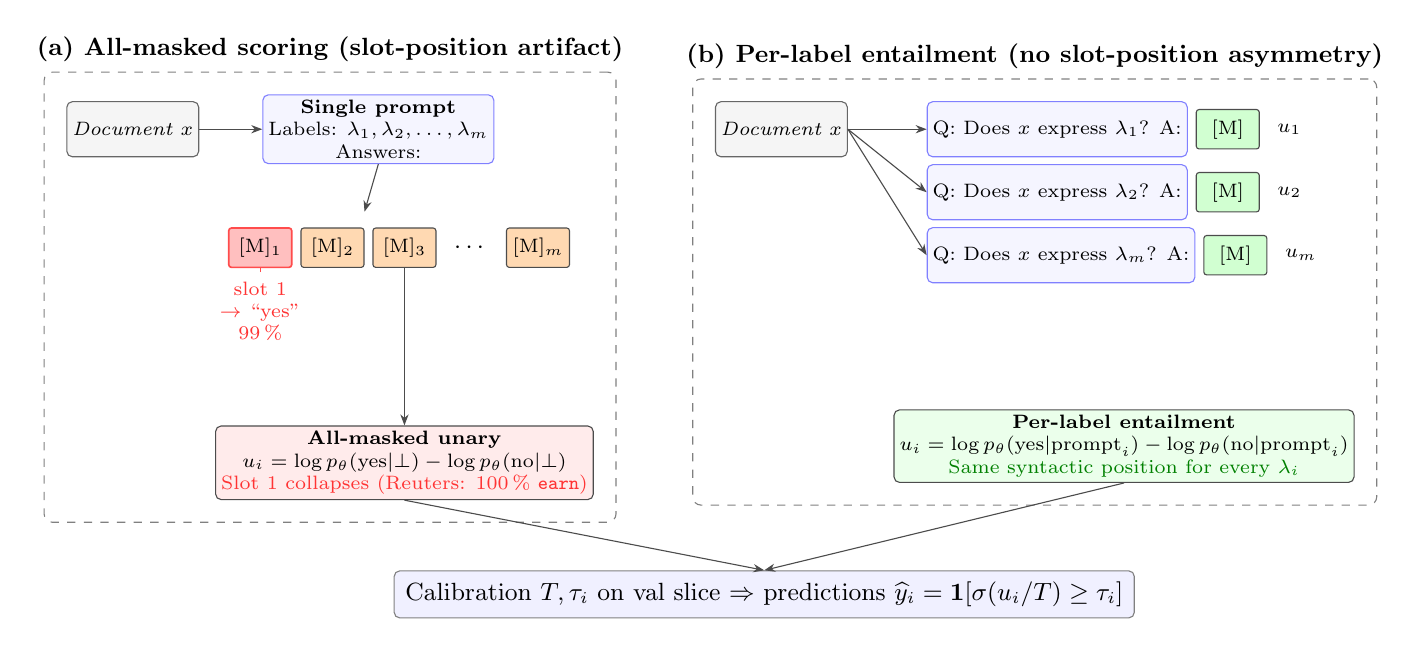
\begin{tikzpicture}[
  font=\small,
  node distance=3mm and 4mm,
  prompt/.style={draw=blue!50, fill=blue!4, rounded corners=2pt, inner sep=2pt, minimum height=7mm, align=center, font=\scriptsize},
  doc/.style={draw=black!60, fill=gray!8, rounded corners=2pt, inner sep=2pt, minimum height=7mm, align=center, font=\scriptsize\itshape},
  slot/.style={draw=black!70, rounded corners=1pt, minimum width=8mm, minimum height=5mm, inner sep=1pt, align=center, font=\scriptsize, fill=white},
  slotmask/.style={slot, fill=orange!30},
  slotbias/.style={slot, fill=red!25, draw=red!70, line width=0.6pt},
  slotok/.style={slot, fill=green!18},
  arrow/.style={-{Stealth[length=1.4mm]}, draw=black!70},
  scoreout/.style={draw=black!70, fill=yellow!12, rounded corners=2pt, inner sep=2pt, minimum height=7mm, align=center, font=\scriptsize},
  modebox/.style={draw=black!50, dashed, rounded corners=3pt, inner sep=3pt},
]
\node[doc] (docL) {Document $x$};
\node[prompt, right=8mm of docL] (instrL) {\textbf{Single prompt}\\Labels: $\lambda_1,\lambda_2,\ldots,\lambda_m$\\Answers:};
\draw[arrow] (docL.east) -- (instrL.west);
\node[slotbias, below=8mm of instrL.south, xshift=-15mm] (m1) {[M]$_1$};
\node[slotmask, right=1mm of m1] (m2) {[M]$_2$};
\node[slotmask, right=1mm of m2] (m3) {[M]$_3$};
\node[right=1mm of m3] (mdotsL) {$\cdots$};
\node[slotmask, right=1mm of mdotsL] (mm) {[M]$_m$};
\draw[arrow] (instrL.south) -- ($(m2.north east)+(0,2mm)$);
\node[font=\scriptsize\color{red!80}, below=0.5mm of m1, align=center] (collapse) {slot 1\\$\to$ ``yes''\\99\,\%};
\draw[red!70, dashed] (collapse.north) -- (m1.south);
\node[scoreout, below=20mm of m3, fill=red!8] (outL) {\textbf{All-masked unary}\\$u_i = \log p_\theta(\text{yes}{\mid}\bot) - \log p_\theta(\text{no}{\mid}\bot)$\\\textcolor{red!80}{\scriptsize Slot 1 collapses (Reuters: 100\,\% \texttt{earn})}};
\draw[arrow] (m3.south) -- (outL.north);
\node[modebox, fit=(docL)(instrL)(mm)(outL)(collapse), inner sep=8pt, label=above:{\bfseries (a) All-masked scoring (slot-position artifact)}] (panelL) {};

\node[doc, right=28mm of instrL.east] (docR) {Document $x$};
\node[prompt, right=10mm of docR.east] (p1) {Q: Does $x$ express $\lambda_1$? A:};
\node[prompt, right=10mm of docR.east, yshift=-8mm] (p2) {Q: Does $x$ express $\lambda_2$? A:};
\node[prompt, right=10mm of docR.east, yshift=-16mm] (pm) {Q: Does $x$ express $\lambda_m$? A:};
\draw[arrow] (docR.east) -- (p1.west);
\draw[arrow] (docR.east) -- (p2.west);
\draw[arrow] (docR.east) -- (pm.west);
\node[slotok, right=1mm of p1] (s1) {[M]};
\node[slotok, right=1mm of p2] (s2) {[M]};
\node[slotok, right=1mm of pm] (sm) {[M]};
\node[font=\scriptsize, right=1mm of s1] {$u_1$};
\node[font=\scriptsize, right=1mm of s2] {$u_2$};
\node[font=\scriptsize, right=1mm of sm] {$u_m$};
\node[scoreout, below=16mm of pm, xshift=8mm, fill=green!8] (outR) {\textbf{Per-label entailment}\\$u_i = \log p_\theta(\text{yes}{\mid}\text{prompt}_i) - \log p_\theta(\text{no}{\mid}\text{prompt}_i)$\\\textcolor{green!50!black}{\scriptsize Same syntactic position for every $\lambda_i$}};
\node[modebox, fit=(docR)(p1)(pm)(sm)(outR), inner sep=8pt, label=above:{\bfseries (b) Per-label entailment (no slot-position asymmetry)}] (panelR) {};

\node[draw=black!50, fill=blue!6, rounded corners=2pt, inner sep=4pt, below=10mm of $(outL.south)!0.5!(outR.south)$, align=center, font=\small] (cal)
  {Calibration $T,\tau_i$ on val slice $\Rightarrow$ predictions $\widehat y_i = \mathbf{1}[\sigma(u_i/T) \ge \tau_i]$};
\draw[arrow] (outL.south) -- (cal.north);
\draw[arrow] (outR.south) -- (cal.north);
\end{tikzpicture}
\end{document}
